\documentclass[pdftex,titlepage]{article}

\author{Noah Santschi-Cooney - 116361061}
\date{8\textsuperscript{th} March 2020}
\title{\textbf{Alternative Visualisation of Distributed Tracing data in a complex, large-scale distributed system}}

\usepackage{graphicx}
\graphicspath{ {./assets/} }

\PassOptionsToPackage{hyphens}{url}\usepackage{url}
\usepackage{microtype}

\begin{document}
    \maketitle
    \section{Introduction}

    Modern Internet services are often implemented as complex, large-scale distributed systems. 
    These applications are constructed from collections of software modules that could span many
    thousands of machines across multiple physical facilities. With the rise of modern 
    Micro-Service and Service-Oriented designs, traditional tooling used to monitor application 
    behaviour is no longer viable, especially at scale\cite{retrospective}. To understanding the flow and lifecycle 
    of a unit of work performed in multiple pieces across various components in a distributed system, 
    the concept of Distributed Tracing was born\cite{xtrace}. 
    
    Distributed Tracing, as it is known today, was first introduced to the mainstream world in 2010 after the publication
    of Google’s Dapper paper\cite{dapper}. Since then, various standards have evolved and numerous vendors have
    come out with their own Dapper-inspired services, most of them utilising visualizations such as
    flame graph or timeline graphs. This final year project aims to explore ways of leveraging modern 
    distributed tracing standards to create novel ways of consuming the outputs of instrumented applications.

    \section{Distributed Tracing}
    The concept of distributed tracing has existed for over a decade at the time of writing. 
    This section will provide a brief history and overview of the main concepts and implementations of distributed tracing,
    from the first published paper of the implementation at Google to modern day standards.

        \subsection{Dapper}
        Released in April 2010, Google published a paper describing the design decisions behind an in-house implementation 
        of distributed tracing, named Dapper. It is commonly believed that this paper describes the common ancestor to 
        many tools that implement a form of distributed tracing.

        The Dapper paper introduces some of the core primitives that underpin modern day standards. Most notable are the concepts
        of a directed acyclic graph (DAG) called a \textit{trace tree} and its nodes, which are referred to as \textit{spans}. 
        The trace tree forms a relationship between spans, not unakin to a tree of stack frames that may be generated by
        gathering stack frames over time, albeit generally at a much higher level than at the level of individual subroutine calls. 

        Figure~\ref{fig:dappertrace} illustrates a trace tree with five spans. Each span is shown to contain 3 specific pieces of
        metadata alongside the start and end timestamps necessarily to reconstruct the temporal relationships: a human-readable
        \textit{span name}, an integer \textit{span ID} and an integer \textit{parent ID}. The latter two
        data points are used to reconstruct the relationship between individual spans. A span without a parent ID becomes the 
        \textit{root span} of a trace tree. Not shown is another important but, as of right now, not relevant piece of metadata, the 
        \textit{trace ID}, which is common amongst all spans within a single trace tree.

        \begin{figure}[htb!]
            \centering
            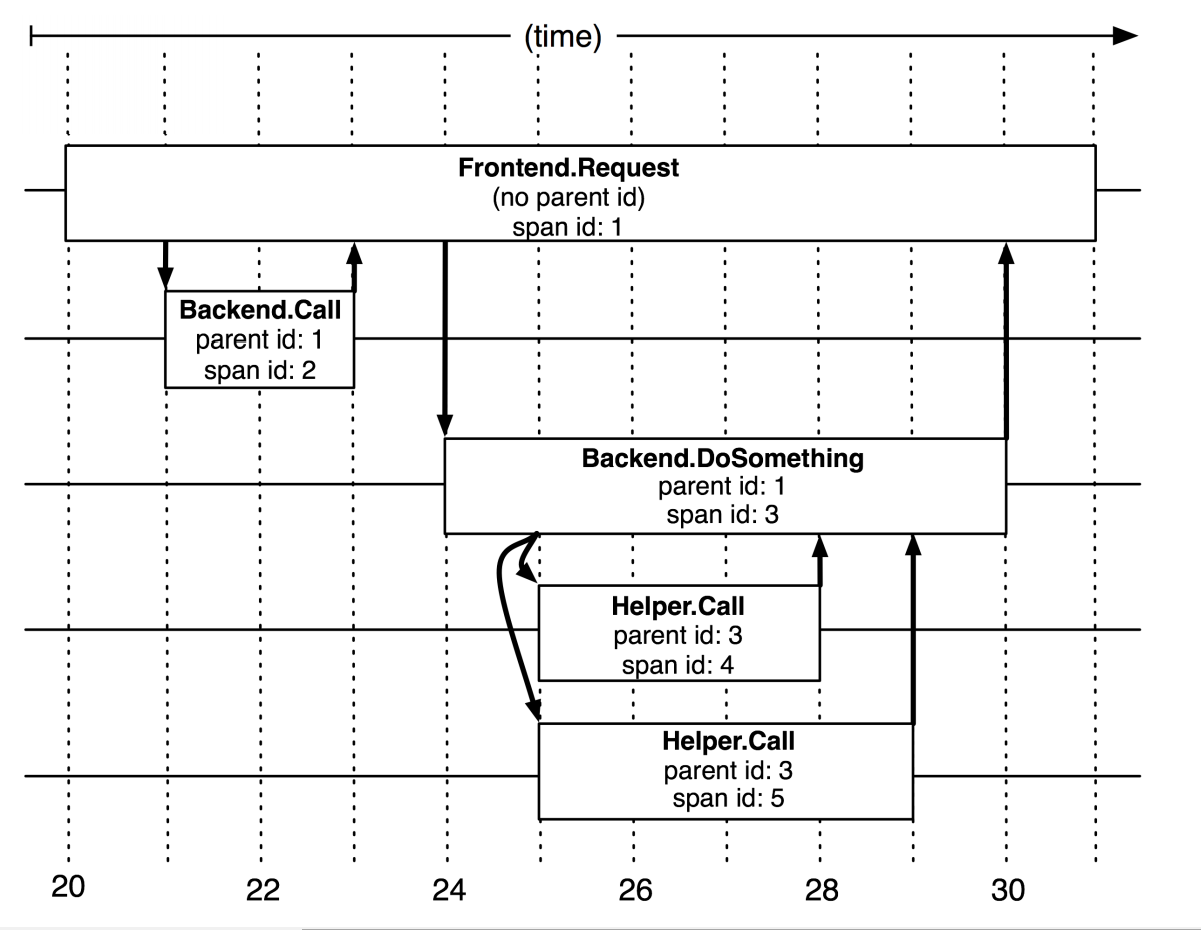
\includegraphics[scale=0.9]{dappertrace}
            \caption{The relationships between traces in a trace tree.}
            \label{fig:dappertrace}
        \end{figure}

        As described thus far, Dapper trace trees allow for a detailed view of the relationships of distributed systems within
        Google. When using this data for debugging or performance analysis, it can often be convenient or even necessary to 
        have additional context surrounding a trace tree or its individual spans. As such, the paper describes a simple API 
        through which application developers can provide a combination of two types of annotations: timestamped textual annotations
        and key-value, allowing for defining arbitrary equivalence classes between traces which can be operated upon in the analysis
        tools.

        \subsection{OpenTracing}
        OpenTracing\cite{opentracing} project's inception came about in October 2015, it has since become a project under the 
        Cloud Native Computing Foundation in 2016, created to standardize a set of vendor neutral and programming language agnostic
        application programming interfaces (APIs) for instrumenting code for distributed tracing. Heavily inspired by the Dapper
        paper, it borrows many of the nouns and verbs outlined in the Dapper paper, including \textit{traces} and \textit{spans}.
        Dapper's timestamped annotations are referred to as \textit{logs} in the OpenTracing specification, while the key-value pairs
        are named \textit{tags}. 

        The OpenTracing API also specifies how a trace cross process boundaries, so that spans created in different processes can be
        associated with a common trace tree. This was named the \textit{span context} and at it's most basic level contains the 
        overlying trace ID as well as the current span ID. With this, new spans generated across process boundaries have the ability to
        to specify their parent span as well as their common trace, without propagating an entire span, which may prove costly as more
        tags and logs are attached to a span.
        
    \section{Visualizations of Distributed Tracing Data}
    All this telemetry data would be of little use if it wasn't consumed in some manner. As distributed tracing has only become a more
    prominent topic in the industry in the last half decade, the set of visualizations that exist and are commonly employed is still rather
    small in number. In this section, we will discuss some of the most common forms of visualizations, leading up to the methods explored 
    in this project.
    
        \subsection{Flame Graph}
        By far the most commonly adopted visualization is a style of graph closely modeled after the \textit{flame graph}\cite{lightsteptrace}
        \cite{datadogtrace} style, closely resembling Figure~\ref{fig:dappertrace}. It also goes under various other names, 
        examples ranging from \textit{gantt chart}\cite{yuritrace} to \textit{waterfall view}\cite{honeycombtrace}. An example of 
        such can be seen in Figure~\ref{fig:jaeger}. Each entry in the graph corresponds to a span in the overall trace tree. They 
        can be expanded to provide the logs and tags associated with a given span. The value that can be derived from this visualization
        has resulted in large adoption of the flame graph style in distributed tracing providers and platforms, leading many to consider
        it the de-facto visualization option for tracing data.

        \medskip

        \begin{figure}[htb!]
            \centering
            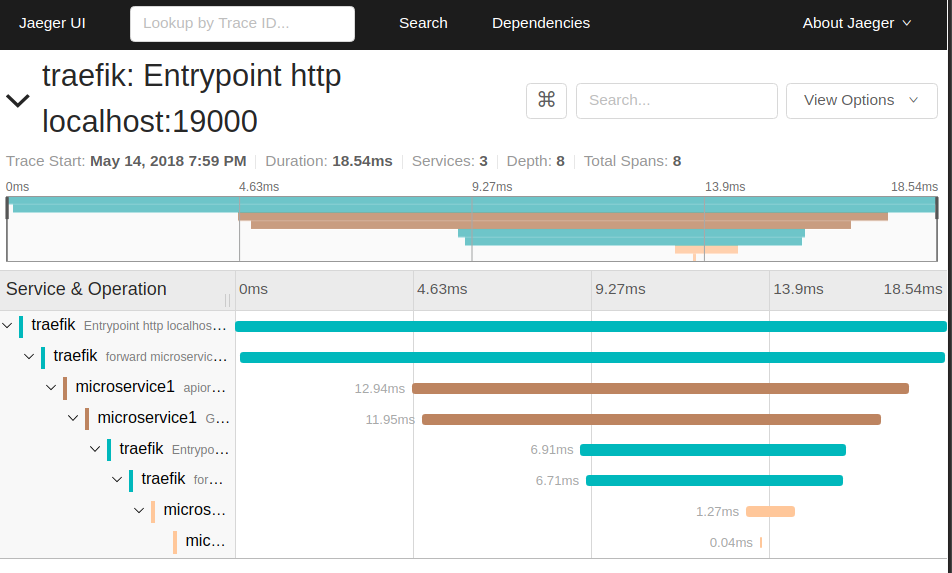
\includegraphics[scale=0.35]{jaeger}
            \caption{Example of the visualization of tracing data in Uber's Distributed Tracing platform, Jaeger\cite{jaeger}.}
            \label{fig:jaeger}
        \end{figure}

        \subsection{Scatter Plot Graph}
        Less commonly found is the traditional \textit{scatter plot graph}, with trace duration on the \textit{y}-axis
        and time on the \textit{x}-axis. This is often complementary to an overview list of all collected traces, which
        facilitates singling out notably longer in duration traces which may be of particular interest in debugging production
        slow-downs\cite{jaegerscatter}\cite{newrelicscatter}\cite{kialiscatter}.

        \subsection{Service Topology}
        This was the first alternative explored as part of the final year project. Since deciding to pursue this type of visualization,
        it had become more widespread in its adoption between different vendors\cite{risingstacktopo}\cite{kialitopo}. Most commonly, 
        a force-directed graph is employed for its aesthetically pleasing properties.

        A basic service topology graph can give a quick overview of the dependencies between different services in a distributed
        system. However, it has little use outside of making ones boss happy. For developers and administrators to derive tangible
        value from such a visualization, there is a need for a more dynamic system. The ability to generate views based on arbitrary
        attributes would allow for users of the system to create more personalized and focused graphs based on their needs,
        such as grouping by high cardinality fields like end-user IP address, error rates, response times etc\cite{doingitwrongtopo}.

        The aim of this section of the project was to explore the viability and value of creating such a system, with the addition
        of being able to replay individual traces instead of being presented an aggregated view. This took inspiration from the
        Massachusetts Bay Transit Authority (MBTA) data visualization project\cite{mbta}.

        \subsection{In-Editor Debugger Integration}
        This is the second and final alternative explored as part of the project. The goal of this visualization alternative was to
        experiment with the attaching of runtime information to the tags of spans and processing said data in such a way that in-editor
        debugging tools can consume it to step through code akin to attaching to a local process using the same debugging tools.

        Unlike traditional debuggers such as the \textit{GNU Project Debugger} (gdb), where stepping through code requires complete
        halting of program execution, using the runtime data attached to trace data allows for after-the-fact, non-blocking stepping
        through code, at an expectedly lower resolution than what can be achieved through traditional, halting debuggers.

        The end goal for this method is to be able to jump between different services' codebases located on a developers local machine,
        where each codebase would be a different microservice in a distributed system. 

    \newpage

    \section{Outcomes}

    The extended service topology visualization was the first alternative visualization that was attempted. The hoped outcome for this was 
    to create a novel way to visualize the timings of events within a trace in relation to other concurrent traces, in ways inspired by 
    the aforementioned MBTA visualization  project. Unfortunately due to complications in the trialing of libraries and the increase of 
    3rd party services providing similarly improved visualizations\cite{risingstacktopo}\cite{kialitopo}, the decision was made to allocate
    more resources to pursuing the second idea for visualization.

    For the in-editor debugger integration, it is planned to support both mono-repos (multiple service codebases in a single version-controlled
    system) as well poly-repos, as well as a multitude of different programming languages. At the time of writing, both Golang and Rust have been
    trialed, with more extensive attempts made in the former with acceptable results. Current efforts revolve around support for Microsoft's
    \textit{Visual Studio Code} editor, however future work could involve porting functionality for other editors or \textit{integrated development
    environments} (IDEs).

    As many languages, especially compiled, do not support retrieving a list of currently defined variables without relying on information baked
    into the binary, we rely on developers to adequately contextualize their traces and spans with aforementioned tags and log points. These 
    can be displayed in the debugger panel where one might usually find the stack and heap variables that a traditional debugger would be able
    to derive.

    Finally, it is hoped that by the end of the project's time period, it will be possible to step through code of polyglottal 
    microservices\cite{polyglot}. As local codebases may be located in a vast variety of locations from developer to developer, there must be a
    means of mapping the services each span is associated with as well as the location in code of the current span with the local location of 
    the codebase on the developers machine. For simplicity's sake, the number of edge cases considered will be reduced, with a focus on the 
    green path, where the only span emitters are instrumented with the code created as part of this project as well as assuming that 3rd party
    code is not instrumented to emit tracing data.

    \begin{thebibliography}{20}
        \bibitem{retrospective}
        Charity Majors, \textit{Observability - A 3-Year Retrospective.} 
        The New Stack, 6th Aug 2019 \\
        \url{https://thenewstack.io/observability-a-3-year-retrospective/}
        
        \bibitem{xtrace}
        Rodrigo Fonseca, George Porter, Randy H. Katz, Scott Shenker \\
        \textit{X-Trace: A Pervasive Network Tracing Framework.} \\
        Cambridge, MA. April 2007 \\
        \url{https://www.usenix.org/conference/nsdi-07/x-trace-pervasive-network-tracing-framework}

        \bibitem{dapper}
        Benjamin H. Sigelman, Luiz André Barroso, Mike Burrows, Pat Stephenson, Manoj Plakal, Donald Beaver, Saul Jaspan, Chandan Shanbhag, \\
        \textit{Dapper, a Large-Scale Distributed Systems Tracing Infrastructure.} \\
        Google, Inc. 2010 \\
        \url{https://research.google/pubs/pub36356/}

        \bibitem{mbta}
        Mike Barry, Brian Card, \textit{Visualizing MBTA Data.}
        10th June 2014 \\
        \url{https://mbtaviz.github.io/}

        \bibitem{opentracing}
        Benjamin H. Sigelman (co creator), \textit{The OpenTracing project.}
        October 2015 \\
        \url{https://opentracing.io/}

        \bibitem{jaeger}
        Yuri Shkuro, \textit{Jaeger, a Distributed Tracing Platform.}
        Uber, April 2016 \\
        \url{https://www.jaegertracing.io/}

        \bibitem{jaegerscatter}
        \textit{Jaeger Scatter Plot Graph configuration.} \\
        \url{https://www.jaegertracing.io/docs/1.17/frontend-ui/#configuration-options}

        \bibitem{newrelicscatter}
        \textit{New Relic Scatter Plot example.} \\
        \url{https://docs.newrelic.com/docs/apm/distributed-tracing/ui-data/understand-use-distributed-tracing-data#}

        \bibitem{kialiscatter}
        \textit{Kiali Scatter Plot view.} \\
        \url{https://kiali.io/documentation/distributed-tracing/#_tracing_view}

        \bibitem{risingstacktopo}
        Gergely Nemeth, \textit{RisingStack Service Topology Graph.} \\
        Rising Stack, 5th May 2016 \\
        \url{https://blog.risingstack.com/distributed-transaction-tracing-microservices-monitoring/#microservicestopology}

        \bibitem{kialitopo}
        \textit{Kiali Service Mesh based Topology Graph.} \\
        \url{https://kiali.io/documentation/features/#_graph}

        \bibitem{doingitwrongtopo}
        Cindy Sridharan, \textit{Distributed Tracing - we've been doing it wrong.} \\
        Medium, 2nd July 2019 \\
        \url{https://medium.com/@copyconstruct/distributed-tracing-weve-been-doing-it-wrong-39fc92a857df}

        \bibitem{polyglot}
        Lianping Chen, \textit{Microservices: Architecting for Continuous Delivery and DevOps.} \\
        March 2018 \\
        \url{https://www.researchgate.net/publication/323944215_Microservices_Architecting_for_Continuous_Delivery_and_DevOps}

        \bibitem{datadogtrace}
        Brad Menezes, \textit{Datadog + OpenTracing: Embracing the open standard for APM.} \\
        DataDog, 6th December 2017 \\
        \url{https://www.datadoghq.com/blog/opentracing-datadog-cncf/}

        \bibitem{honeycombtrace}
        \textit{Explore trace data documentation.} \\
        Honeycomb.io \\
        \url{https://docs.honeycomb.io/working-with-your-data/tracing/explore-trace-data/#using-the-waterfall-view}

        \bibitem{lightsteptrace}
        \textit{View Traces documentation}
        Lightstep \\ 
        \url{https://docs.lightstep.com/docs/view-traces}

        \bibitem{yuritrace}
        Yuri Shkuro, \textit{Mastering Distributed Tracing.} \\
        Packt, February 2019 \\
        \url{https://www.packtpub.com/eu/networking-and-servers/mastering-distributed-tracing}
    \end{thebibliography}
\end{document}